Des programmes de tests ont été appliqués à notre bibliothèque. Ceux qui acceptent un argument en paramètre ne marchent plus essayés avec un argument trop grand, ceci est en général dû à l'allocation de mémoire avec \textbf{malloc} dans le tas. Ceci dépend bien sûr des capacités de la machine sur laquelle le test a eu lieu.
Tous les tests qui suivent ont été réalisés sur une machine virtuelle comportant 3 Go de mémoire vive, 2 coeurs tournant à 2.2 GHz:\\

\begin{itemize}

\item Les tests \textbf{exemple}, \textbf{join}, \textbf{main} , \textbf{join-main} et \textbf{switch} tournent correctement. \\

\item Le test \textbf{create-many} marche avec un argument pouvant aller jusqu'aux alentours de 5000000, c'est-à-dire 5000000 threads créés puis détruits. On peut augmenter même plus mais le temps d'exécution devient alors très élevé. \\
La figure suivante montre une comparaison entre les performances de notre bibliothèque pour ce test, et les performances de la bibliothèque standard:\\
\begin{figure}[h!]
\centering
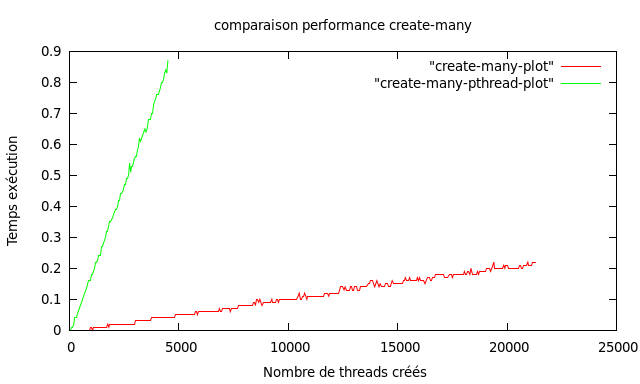
\includegraphics[width=120mm]{create-many.png}
%\caption{Figure 1}
\end{figure}

Comme nous le montre la figure, notre bibliothèque est plus rapide, c'est d'ailleurs pour cette raison que les tests avec les \textbf{pthread} ont été arrétés avec un argument beaucoup plus petit que ceux avec notre bibliothèque.\\
\item Le test \textbf{create-many-recursif} accepte un argument allant jusqu'à 45000. Au-delà de cette valeur, le temps d'exécution et soit trop élevé, soit c'est le caractère récursif de la fonction qui a donc une complexité en espace assez élevée ce qui bloque le déroulement du programme.\\
La figure suivante montre une comparaison entre les performances de notre bibliothèque pour ce test, et les performances de la bibliothèque standard:\\
\begin{figure}[h!]
\centering
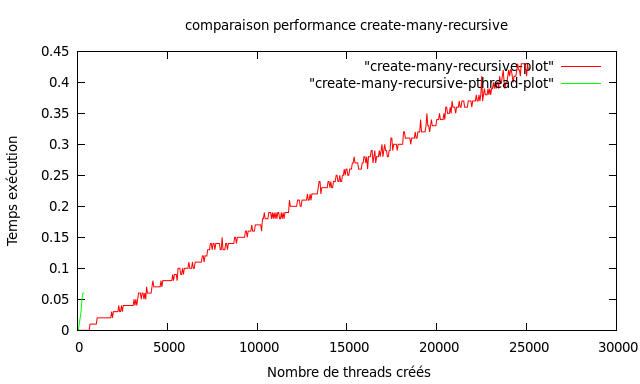
\includegraphics[width=120mm]{create-many-recursive.png}
%\caption{Figure 1}
\end{figure}

La vitesse du test utilisé avec notre bibliothèque étant plus élévée que celle du test avec les \textbf{pthread}, la taille de l'argument a été très vite limitée. La courbe verte, représentant le temps d'exécution en fonction de l'argument pour les tests avec les \textbf{pthread} montre une pente assez élévée et donc un temps d'exécution qui augmente très vite avec la taille de l'argument.\\
\item Le test \textbf{fibonacci} ne peut être exécuté avec un argument de valeur supérieure à 23. Au-delà de cette valeur, on a une erreur d'allocation: on ne peut plus allouer de la mémoire. Avec les \textbf{pthread} cette valeur ne peut dépasser 12.\\
La figure suivante montre une comparaison entre les performances de notre bibliothèque pour ce test, et les performances de la bibliothèque standard:\\
\newpage
\begin{figure}[h!]
\centering
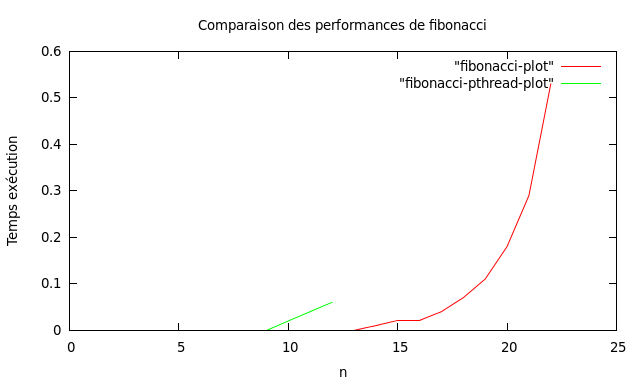
\includegraphics[width=120mm]{fibonacci.png}
%\caption{Figure 1}
\end{figure}

La figure nous montre un temps d'exécution nul pour les tests avec les \textbf{pthread} jusqu'à un argument égal à 9. Ensuite cette valeur augmente de façon linéaire. Par contre, les tests faits avec notre bibliothèque ont un temps d'exécution nul jusqu'à un argument de valeur 13 puis augmente considérablement jusqu'à atteindre l'argument maximal, 23. Notre bibliothèque est donc plus rapide que la bibliothèque standard.\\
\item Le test \textbf{switch-many} tourne correctement avec un nombre élevé de threads (4000 threads) et un nombre élevé de yields (4000 yields). On peut considérablement augmenter le nombre de threads (jusqu'à 40000), par contre, dès que le nombre de yields augmente, le temps d'exécution devient trop long, déjà que pour 4000 threads et 4000 yields, le temps d'exécution dépasse les 10 secondes. \\
\item Le test \textbf{switch-many-join} tourne correctement avec un nombre élevé de threads (45000 threads) et un nombre très élevé de yields (200000 yields).\\

\end{itemize}